\section{Experiment}
\label{sec:experiment}

In this section, we describe empirical experiments that recommend a set of music using the proposed methods
described in Section~\ref{sec:method}, and compare with a few well known baseline approaches.

\subsection{Music playlist dataset}
We make use of two publicly available playlist dataset: the AotM-2011~\cite{mcfee2012hypergraph} and 30Music~\cite{30music2015} playlist dataset.
The Million Song Dataset~\cite{msd2011} serves as an underline dataset where all songs in playlists are intersected with,
it also provides a few features of songs which we will detail later.

{\bf Million Song Dataset} (MSD) is a collection of one million songs, information of each song such as the name, artist, year of release are available.
It also provides acoustic features computed from a sample section of audio file for each song. % more description

{\bf AotM-2011 Dataset} is a collection of playlists shared by users\footnote{\url{http://www.artofthemix.org}} ranging from 1998 to 2011, 
songs in the dataset had been matched to those in the Million Song Dataset (MSD).
We filtered out playlists with less than 5 songs, which results in roughly 84K playlists over 114K songs from 14K users.

{\bf 30Music Dataset} is a collection of listening events and playlists retrieved from Last.fm\footnote{\url{https://www.last.fm}}.
We utilise the playlists data by first intersecting with the MSD, leveraging the Last.fm dataset~\cite{lastfmdataset} 
which matched songs from Last.fm with those in MSD, then filtering out playlists with less than 5 songs, 
which results in roughly 17K playlists over 45K songs from 8K users.
Table~\ref{tab:stats_pldata} summarises the two playlist dataset used in this work.
%
\begin{table}[!h]
\centering
\caption{Statistics of music playlist dataset}
\label{tab:stats_pldata}
\resizebox{\linewidth}{!}{
\small
\begin{tabular}{lrcrcc}
\toprule
Dataset   & Songs & Playlists & Users & Songs/Playlist & Playlists/User \\
\midrule
AotM-2011 & 114,428 & 84,710  & 14,182  & 10.1 & 6.0 \\
30Music   & 45,468  & 17,457  & 8,070   & 16.3 & 2.2 \\
\bottomrule
\end{tabular}
}
\end{table}



\subsection{Experimental setup}
We describe the how playlist data are split in training and test set,
features of songs used to learn the multitask objective, baseline approaches 
and evaluation metrics.

{\bf Dataset split}.
To empirically evaluate the performance of our proposed recommendation approaches for existing users,
we hold playlists from about 20\% users in AotM-2011 and 30Music dataset for test,
all other playlists are used for training.
To make sure each song in test set also appeared in training set, 
and all users in test set also have a few playlists in training set,
The test set are sampled from users that have at least one playlist in which each song has also been
included in five playlists in the whole dataset,
which results in about 9.2K playlists from 2.7K users in AotM-2011 dataset,
and 2.1K playlists from 1.6K users in 30Music dataset as test playlists, respectively.
The statistics of this training/test split can be found in Table~\ref{tab:stats_warm}.

\begin{table}[!h]
\centering
\caption{Statistics of dataset for music recommendation for existing users}
\label{tab:stats_warm}
\begin{tabular}{lrrcrr}
\toprule
\multirow{2}{*}{Dataset}  & \multicolumn{2}{c}{Playlists} && \multicolumn{2}{c}{Users} \\ \cmidrule{2-3} \cmidrule{5-6}
                          & Train & Test && Train & Test \\
\midrule
AotM-2011 & 75,477 & 9,233 && 14,182 & 2,722 \\
30Music   & 15,262 & 2,195 &&  8,070 & 1,644 \\
\bottomrule
\end{tabular}
\end{table}

To evaluate the performance of music recommendation approaches for new users,
we sampled 30\% of all users and hold all their playlists as test set in both datasets.
Similarly, to make sure songs in test set also exist in training set,
a user is not sampled when holding all of her playlists breaks this requirement.
This results in about 8.2K playlists from 4.2K users in AotM-2011 dataset,
and 3.4K playlists from 2.4K users in 30Music dataset for testing, respectively.
The statistics of this training/test split can be found in Table~\ref{tab:stats_cold}.

\begin{table}[!h]
\centering
\caption{Statistics of dataset for music recommendation for new users}
\label{tab:stats_cold}
\begin{tabular}{lrrcrr}
\toprule
\multirow{2}{*}{Dataset}  & \multicolumn{2}{c}{Playlists} && \multicolumn{2}{c}{Users} \\ \cmidrule{2-3} \cmidrule{5-6}
                          & Train & Test && Train & Test \\
\midrule
AotM-2011 & 76,450 & 8,260 && 9,928 & 4,254 \\       
30Music   & 14,067 & 3,390 && 5,649 & 2,421 \\
\bottomrule
\end{tabular}
\end{table}


{\bf Features} of each song used in experiment including metadata, audio data, genre, artist information and song popularity.
Song metadata (\eg duration, year of release) and audio features (\eg loudness, mode, tempo) are provided by MSD.

We also make use of genre data from the Top-MAGD genre dataset~\cite{schindler2012facilitating} 
and tagtraum genre annotations for MSD~\cite{schreiber2015improving} via one-hot encoding.
If the genre data of a song is not available, we use a mean imputation with genre counts of other songs in training set.

To encode artist information, we learned a word2vec\footnote{https://github.com/dav/word2vec} model using sequences of artist names in each playlist,
and finally, song popularity (\ie the number of occurrences of a song in training set) is included as a feature.


{\bf Baselines}.
We compare the performance of our proposed approaches for music recommendation given existing users
with a few baseline approaches that were known to work comparably well on this task.

Firstly, the popularity based ranking method, which scores each song using only its popularity 
(the number of occurrences in all playlists) in training set.
%
Another approach that based on song popularity and artist is the Same Artists - Greatest Hits (SAGH)~\cite{mcfee2012million} method,
which scores each song by its popularity if the artist of the song has been appeared in the given user's playlist in training set, 
otherwise the song is scored zero.
%
The Collocated Artists - Greatest Hits (CAGH)~\cite{bonnin2013evaluating} method is closely related to SAGH,
it also scores each song using it popularity, but weighted by the frequency of the collocation between artist of the song 
and those artists that appeared in the given user's playlist in training set.

The popularity based ranking approach is readily available to be a baseline for the setting of recommending music for new users.
%
We slightly modified the SAGH and CAGH approaches so that they can also work in this setting,
in particular, we replace artists that appeared in user's training playlists in the previous setting with the 10 most popular artists
(we use the number occurrences of all songs from a artist in training playlists as a proxy of artist popularity),
and refer these two approaches as Top10 SAGH and Top10 CAGH, respectively.


{\bf Evaluation}.
We evaluate performance of all approaches using three metrics that are commonly employed in music recommendation for playlist tasks:
R-Precision~\cite{manning2008introIR}, Hit-Rate@K~\cite{hariri2012context} and Area under the ROC curve (AUC)~\cite{manning2008introIR}.

R-Precision (RPREC) is the number of correctly recommended songs in the top-$n$ recommendation over $n$,
where $n$ is the number of songs in the ground truth playlist.
It is one of several metrics used to evaluate performance on playlist continuation tasks 
in the ACM RecSys Challenge 2018\footnote{https://recsys-challenge.spotify.com/rules}.
%
Hit-Rate@K (or Hit Ratio) is the number of correctly recommended songs among top-$K$ recommendation over $n$,
where $K$ is the number of recommendations, and $n$ is the number of songs in the ground truth playlist as before.
It has been employed to evaluate several playlist generation and next song recommendation 
methods~\cite{hariri2012context,bonnin2013evaluating,bonnin2015automated,jannach2015beyond}.
%
The area under the ROC curve (AUC) is widely used in measuring performance of classifiers,
it has also been used for evaluating performance of playlist generation method when the task
is cast as a sequential classification problem~\cite{ben2017groove}.



\subsection{Results}

\begin{table}[!h]
\centering
\caption{Performance (given known user) in terms of R-Precision ($\times 10^2$)}
\label{tab:perf_plgen1_r-precision}
\begin{tabular}{l*{4}{c}*{4}{c}}
\toprule
Method     & AotM-2011 & 30Music \\
\midrule
Popularity Rank &     $1.0$ &   $2.2$ \\
SAGH &     $1.5$ &   $4.5$ \\
CAGH &     $1.4$ &   $4.4$ \\
Multitask Classification &       N/A &   $4.8$ \\
Multitask Ranking &       N/A &     N/A \\
\bottomrule
\end{tabular}
\end{table}


\begin{figure}[!h]
\centering
%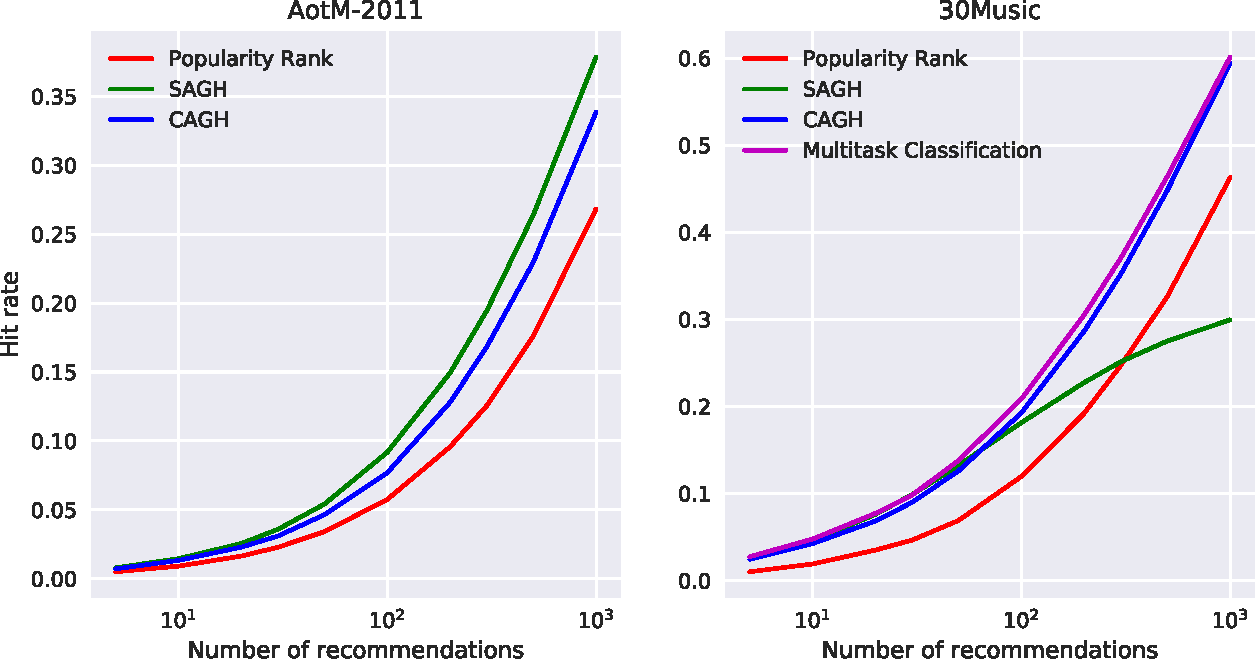
\includegraphics[width=\linewidth]{fig/hitrate-plgen1.pdf}
\caption{Hit rates given known users.}
\end{figure}

\begin{table}[!h]
\centering
\caption{Performance (given new user) in terms of R-Precision ($\times 10^2$)}
\label{tab:perf_plgen2_r-precision}
\begin{tabular}{l*{4}{c}*{4}{c}}
\toprule
Method     & AotM-2011 & 30Music \\
\midrule
Popularity Rank &     $1.3$ &   $2.1$ \\
Top10 SAGH &     $1.2$ &   $2.0$ \\
Top10 CAGH &     $1.2$ &   $2.0$ \\
Multitask Classification &       N/A &   $2.1$ \\
Multitask Ranking &       N/A &     N/A \\
\bottomrule
\end{tabular}
\end{table}


\begin{figure}[!h]
\centering
%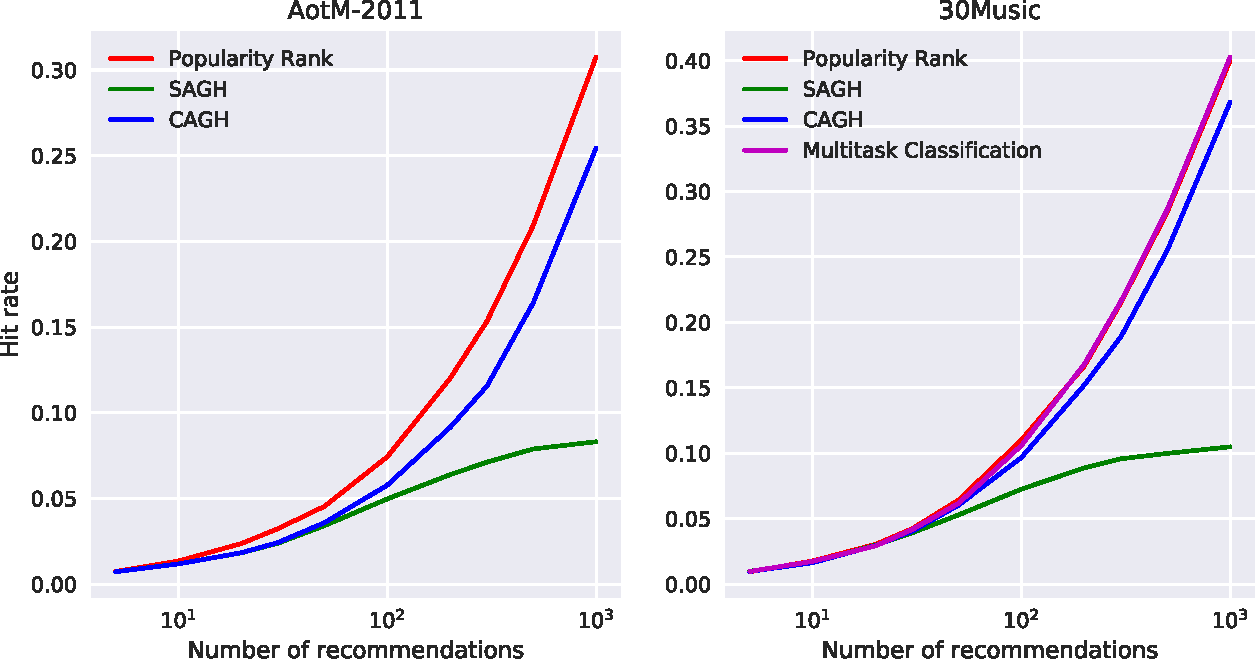
\includegraphics[width=\linewidth]{fig/hitrate-plgen2.pdf}
\caption{Hit rates given new users.}
\end{figure}


\subsection{Discussion}

Data sparsity

Number of parameters in proposed methods are large

Evaluation is challenging.
We believe that promising automatic evaluation methods that accepted by the (majority of) community need to be 
developed before significant progress being made.
